\chapter{Реализация программного продукта}

В данном разделе приводятся измененный алгоритм поведения Виртуального Актора.

\section{Текущая версия реализованной модели}

Для решения задачи разработки экспериментальной платформы на базе виртуального окружения для изучения социально – эмоционального поведения 
акторов целесообразно использовать специальные программные окружения для разработки виртуальных окружений и сопутствующих компонент – «игровые движки». 
По результатам анализа стало понятно, что такая среда должна прежде всего обладать:

\begin{enumerate}
  \item Большим сообществом разработчиков
  \item Подробной документацией
  \item Относительно низкой сложностью
  \item Простотой установки
  \item Модульной системой
\end{enumerate}

Всеми данными свойствами обладает лишь Unity3D, как самый распространённый, на данный момент инструмент построения виртуальных окружений. 
На базе Unity3D сделано больше игр, чем на любой другой технологии, поэтому он и обладает наиболее развитым сообществом разработчиков на данный момент. 
В сети имеется большое множество документации и курсов по данной технологии. Благодаря модульной системе, можно найти специальные программные модули, 
которые легко встраиваются в разработанный продукт, расширяя возможности всей системы.  Преимуществом данной среды также следует считать относительную 
простоту переноса разработанного виртуального окружения на другие платформы (например, смартфоны, планшеты или же любую из существующих операционных систем). 
Также стоит отметить, что программная среда имеет бесплатную лицензионную версию для небольших команд разработчиков.

Unity предлагает разработчику возможность использовать три различных сценарных языка: C\#, JavaScript (его модификация) и Boo (собственный диалект Python). 
Для разработки данной экспериментальной платформы был выбран C\#, как де факто, стандарт при разработке на Unity3D. 

В качестве среды разработки используется Visual Studio 2019. Для контроля версий использовать облачное хранилище Dropbox и GitLab. 
В качестве средства проектирования использовался стандартный модуль Visual Studio для построения диаграмм классов.

\begin{figure}[h]
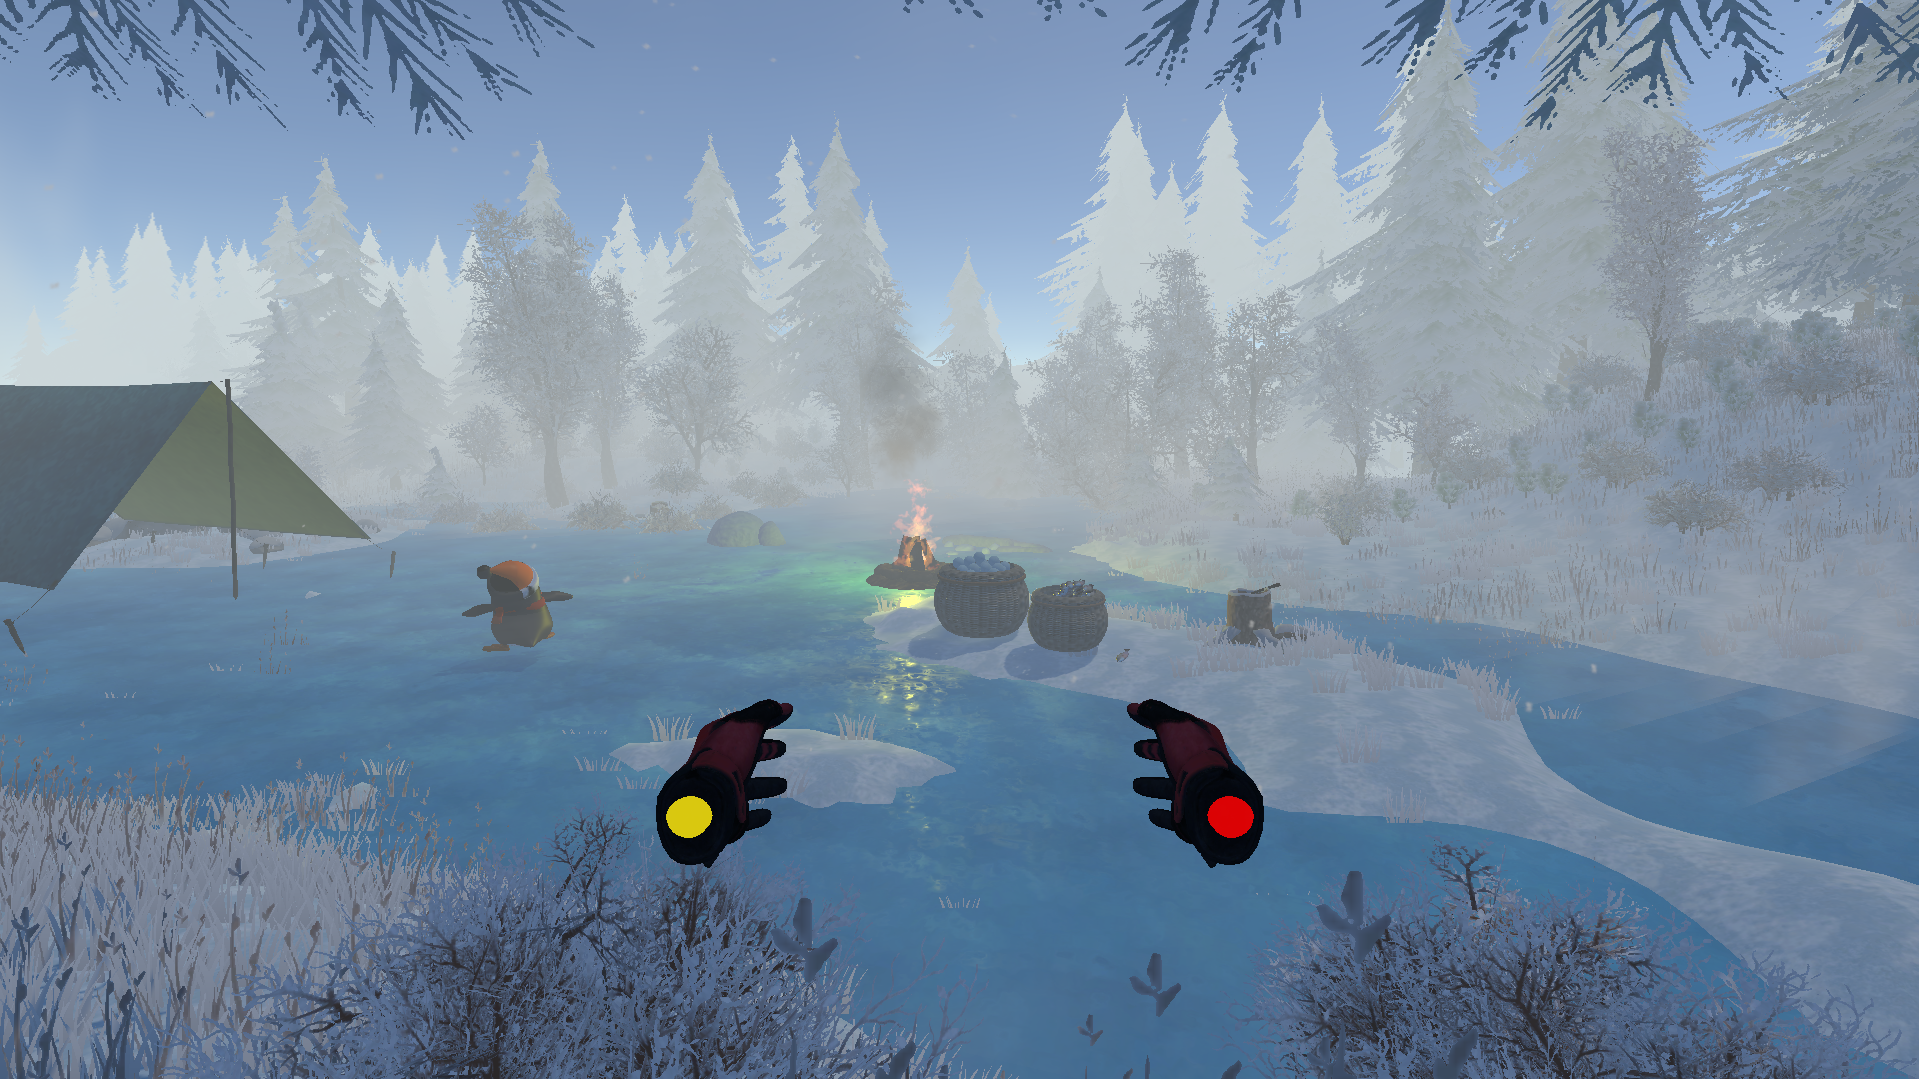
\includegraphics[width=0.75\columnwidth]{./img/penis.png}
\centering
\caption{Cкриншот взаимодействия человека с Виртуальным Актором}
\label{pic:penis}
\end{figure}

В работе было реализовано программное приложени с помощью движка юнити результаты работы которого вы можете видеть на (рис. \ref{pic:penis})

\section{Интеграция моделей из python в C\#}

В расширенной диаграмме классов, было выделено какие стадии обработки проходит аудио-запись (Рис. \ref{pic:ncmodel0}).

Получение Audio из UNITY3D осуществлялось при помощи ксласса Microphone и далее помещалось 
в контейнер для аудио данных AudioClip, который хранит аудиофайл либо сжатым в ogg vorbis, либо без сжатия.

Далее, полученная аудио проходит обработку при помощи моделей реализовнных на языке программирования python, 
при непосредственном использовании IronPython, который представляет из себя реализацию языка программирования 
Python с открытым исходным кодом, которая тесно интегрирована с .NET Framework. 
IronPython может использовать библиотеки .NET Framework и Python, а другие языки .NET могут также легко использовать код Python».

Мы использовали метод ExecuteFile(), так как в нашем случае он самый подходящий.

В указанном выше методе проиходит следующее:
\begin{itemize}
  \item В коде C\# в метод ExecuteFile(@"/home/...") помещен путь к файлу .py
  \item Функция из Python определяется в C\#,
  \item Возвращается результат по заврешнию исполнения кода .py,
\end{itemize}

Таким образом проиходит интеграция реализации динамического языка программирования IronPython в проект.

\section{Команды испольняемые посредством распозавания речи}

Процесс распозавнания речи проводился частично посредством использования 
внутренного инструментария UNITY3D. В нем пакет HoloToolKit Unity
предоставляет несколько методов голосового ввода. В нашем случае был 
выбран метод DictationRecognize который обладает функцией преобразования 
текста в речь. 

Для того чтобы пользователь мог передавать голосовые фразы приложению, следует:

\begin{itemize}
  \item Создать объект DictationRecognize
  \item Произвести инициализацию процесса диктовки
\end{itemize}

Однако HoloToolKit Unity не дает возможности распознавать речь на
русском языке, в связи с чем был использован лишь для сохранения 
аудио в формате ".wav". Сама процедура распознавания речи прводится
с помощью YandexSpeechKit. Для этого был получен уникальный 
IAM-токен для возможности использовать API. Реализовано простое приложение, 
которое получает распознанную речь в формате JSON 

Пример запроса: 

\lstinputlisting[
  float=ht,frame=lines,label=lst:queryjson,caption=Пример запроса
]
{listings/query.json}

Пример ответа: 

\lstinputlisting[
  float=ht,frame=lines,label=lst:queryjson,caption=Пример ответа
]
{listings/answer.json}

Далее посредством определения семантической близости слов по распознанной речи 
выявляются команды для Виртуального Питомца. Полученная последовательность 
команд передается в ActionsAlgothms, где производится временное изменение 
вероятностей выполнения действий. Данные изменения действуют до выполнения 
любого действия, а после сбрасываются. Действие соотносящееся с командной 
повышают свою вероятность исполнения, тогда как остальные понижают. Если 
Действие для которого была передана команда из последовательности командне будет 
выполнена, то остальная часть последовательности не будет провоцировать изменение
в классе ActionsAlgothms. 

Стек возможных команд представлен ниже:

\begin{itemize}
  \item Играть в снежки с человеком 
  \item Играть в снежки с испытуемым
  \item Пищать
  \item Подойти к человеку
  \item Подойти к испытуемому
  \item Пойти спать
  \item Посмотреть в сторону человека
  \item Посмотреть в сторону испытуемого
  \item Поприветствовать человека
  \item Поприветствовать испытуемого
  \item Подойти к корзине с рыбой и поесть
  \item Поесть из рук
\end{itemize}




\section{Реализация и дообучение модели}

Как говорилось ранее для создания возможности эмоционального взаимодействия пользователя с виртуальным актором - 
берется предобученная модель "jonatasgrosman/wav2vec2-large-xlsr-53-russian". Данная модель 
работает в состве библеотки huggingsound. На выходе модели для отдельного аудиофайла получаются 512-мерные вектора. 
Далее высчитывается средней вектор, который передается в модели для распознования эмоций.
Используется python3.8 и библиотека машинного обучения pytorch и sklearn.

Для SVC с ядром RBF менялся параметр регурялизации, а именно он принимал значения 1, 10 и 100.

Для k-NN менялось количество соседей от 10 до 40 с шагом в 10.

Для MLP выходной слой не менялся и состоял из 8 нейронов, тогда как количество внутрених слоев менялось от 1 до 3 так,
что количество нейронов в них оставалось неизменным и равным 1024.
В качестве функции активации была выбрана функция гиперболического тангенса.

Были выделены следющие эмоции для распознавания акустическим методом из речи:

\begin{enumerate}
  \item Злость
  \item Спокойствие
  \item Отвращение
  \item Ужас
  \item Счастье
  \item Нейтральность
  \item Грусть
  \item Удивление
\end{enumerate}

В результате чего был получен следующий результат (таб. \ref{pic:table}): 

\begin{figure}[h]
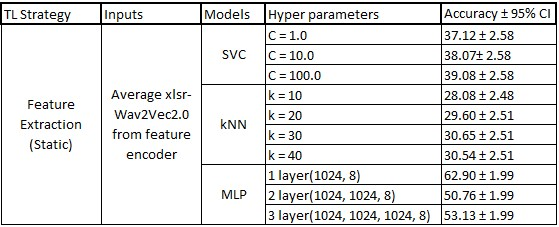
\includegraphics[width=0.75\columnwidth]{./img/table_all_em.jpg}
\centering
\caption{Результаты обучения по 8 выделенным эмоциям}
\label{pic:table}
\end{figure}

Однако результат был не удовлетворительным в связи с чем было принято решение 
упростить классфикацию эмоций на положительные и отрицательные следущим образом (таб. \ref{tbl:em_table}):

\begin{table}[H]
\caption{Разделение эмоций по классам с оценкой}
\label{tbl:text_a00}
\begin{center}
%\centering

\begin{tabular}{ | c | c | c | }
  \hline
  Злость & Отрицательные & -1 \\ \hline 
  Спокойствие & Пололожительные & 1 \\ \hline 
  Овращение & Отрицательные & -1 \\ \hline 
  Ужас & Отрицательные & -1 \\ \hline 
  Счастье & Пололожительные & 1 \\ \hline 
  Нейтральность & Пололожительные & 1 \\ \hline 
  Грусть & Отрицательные & -1 \\ \hline 
  Удивление & Пололожительные & 1 \\ \hline 
\end{tabular}
\end{center}
\end{table}

В соответствии с новым подходом соответствия эмоции одному из двух классов, а именно 
положительному или отрицательному, было получен следующий результат показанный на таблице \ref{pic:table2}:

\begin{figure}[h]
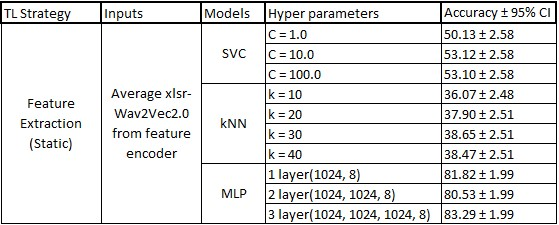
\includegraphics[width=0.75\columnwidth]{./img/table_2_em.jpg}
\centering
\caption{Результаты обучения по классификации эмоций на положительные и отрицательные}
\label{pic:table2}
\end{figure}

В результате чего был получен удовлетврорительный результат.
При обучении датасет разбился на парти в 100 образцов в каждой так, чтобы была возмножность
обучать модели на GPU. Обучение проводилось до 10 эпох так, что результирующей модеью становилась та,
что показывала максимальный результат в какой-либо эпохе.
Так как ставится задача классификации, то в качестве функции потерь используется функция потерь перекрестной энтропии.
В качестве опитимизатора использовался оптимизатор Адам.


\section{Результаты}

В результате было получено следующее взаимодействие, представленное на рисунке \ref{pic:res_actions_plus_voice_actions}:

\begin{figure}[h]
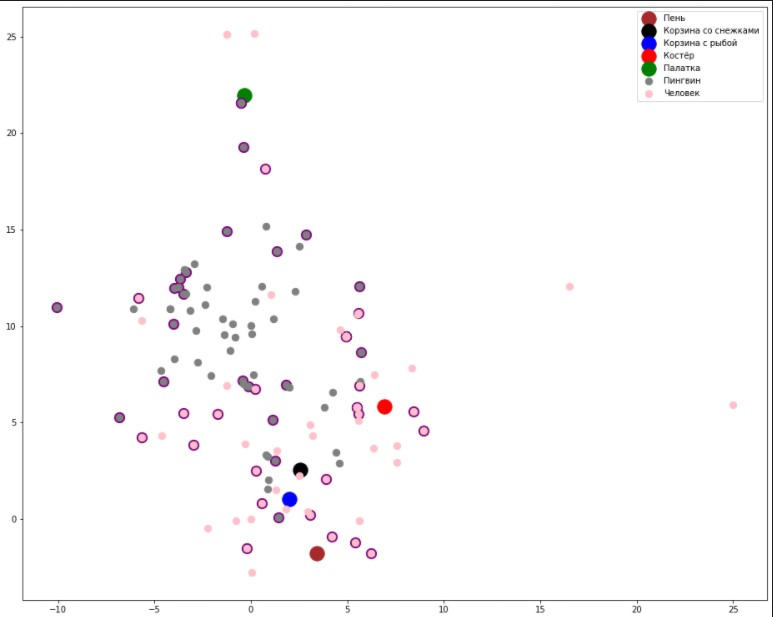
\includegraphics[width=0.75\columnwidth]{./img/res_actions_plus_voice_actions.jpg}
\centering
\caption{Карта перемещений Виртуального Актора и человека}
\label{pic:res_actions_plus_voice_actions}
\end{figure}

Условные обозначения: 

\begin{itemize}
  \item Синий кружок - Корзина с рыбой
  \item Коричневый кружок - Пень
  \item Черный кружок - Корзина со снежками
  \item Красный кружок - Костер
  \item Зеленый кружок - Палатка
  \item Серый кружок - Пингвин
  \item Розовый кружок - Человек
  \item Выделенный кружук фиолетовым - отклик одного из акторов на команду
\end{itemize}

Рисунок предоставляет собой карту где точки находятся на виртуальной сцене 
серым и розовым отмечаются где происходило взаимодейтвия акторов, эти 
места с фиолетовым ободком обозначают, что взаимодейтвие было инициировано
голосовой командой.

\begin{figure}[h]
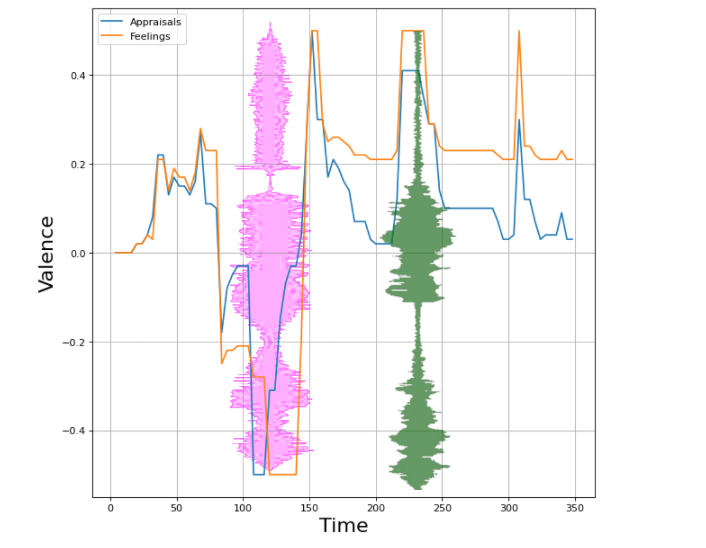
\includegraphics[width=0.75\columnwidth]{./img/GRAFIK.png}
\centering
\caption{Карта перемещений Виртуального Актора и человека}
\label{pic:grafik_res}
\end{figure}

На графике \ref{pic:grafik_res} отображена зависимость Feelings и Appraisals
на шкале Valence от времени, во время эксперимента, по результатам которого 
был построен этот график, было 2 ключевых взаимодействия с испытуемым. Эти
Взаимодействия были классифицированы как отрицательное эмоциональное взаимодействие и положительное.
На графике они изображены рорзовым и зеленым - соответственно.
Из изображения видно, что результат взаимодействия был следующим:
в 110 секунду игровой сессии при было обработано негативное высказывание, что 
оказало влияение на график так что по шкале валентности показатель упал.
Обатное произошло на 231 секунде, когда речевое взаимодействие с виртальным 
вгентом имело позитивный характер.

Фрагменты игровой сессии представлены на риснуках ниже (\ref{draka}, \ref{kormejka}, \ref{nejnost}, \ref{snejok}):

\begin{figure}[h]
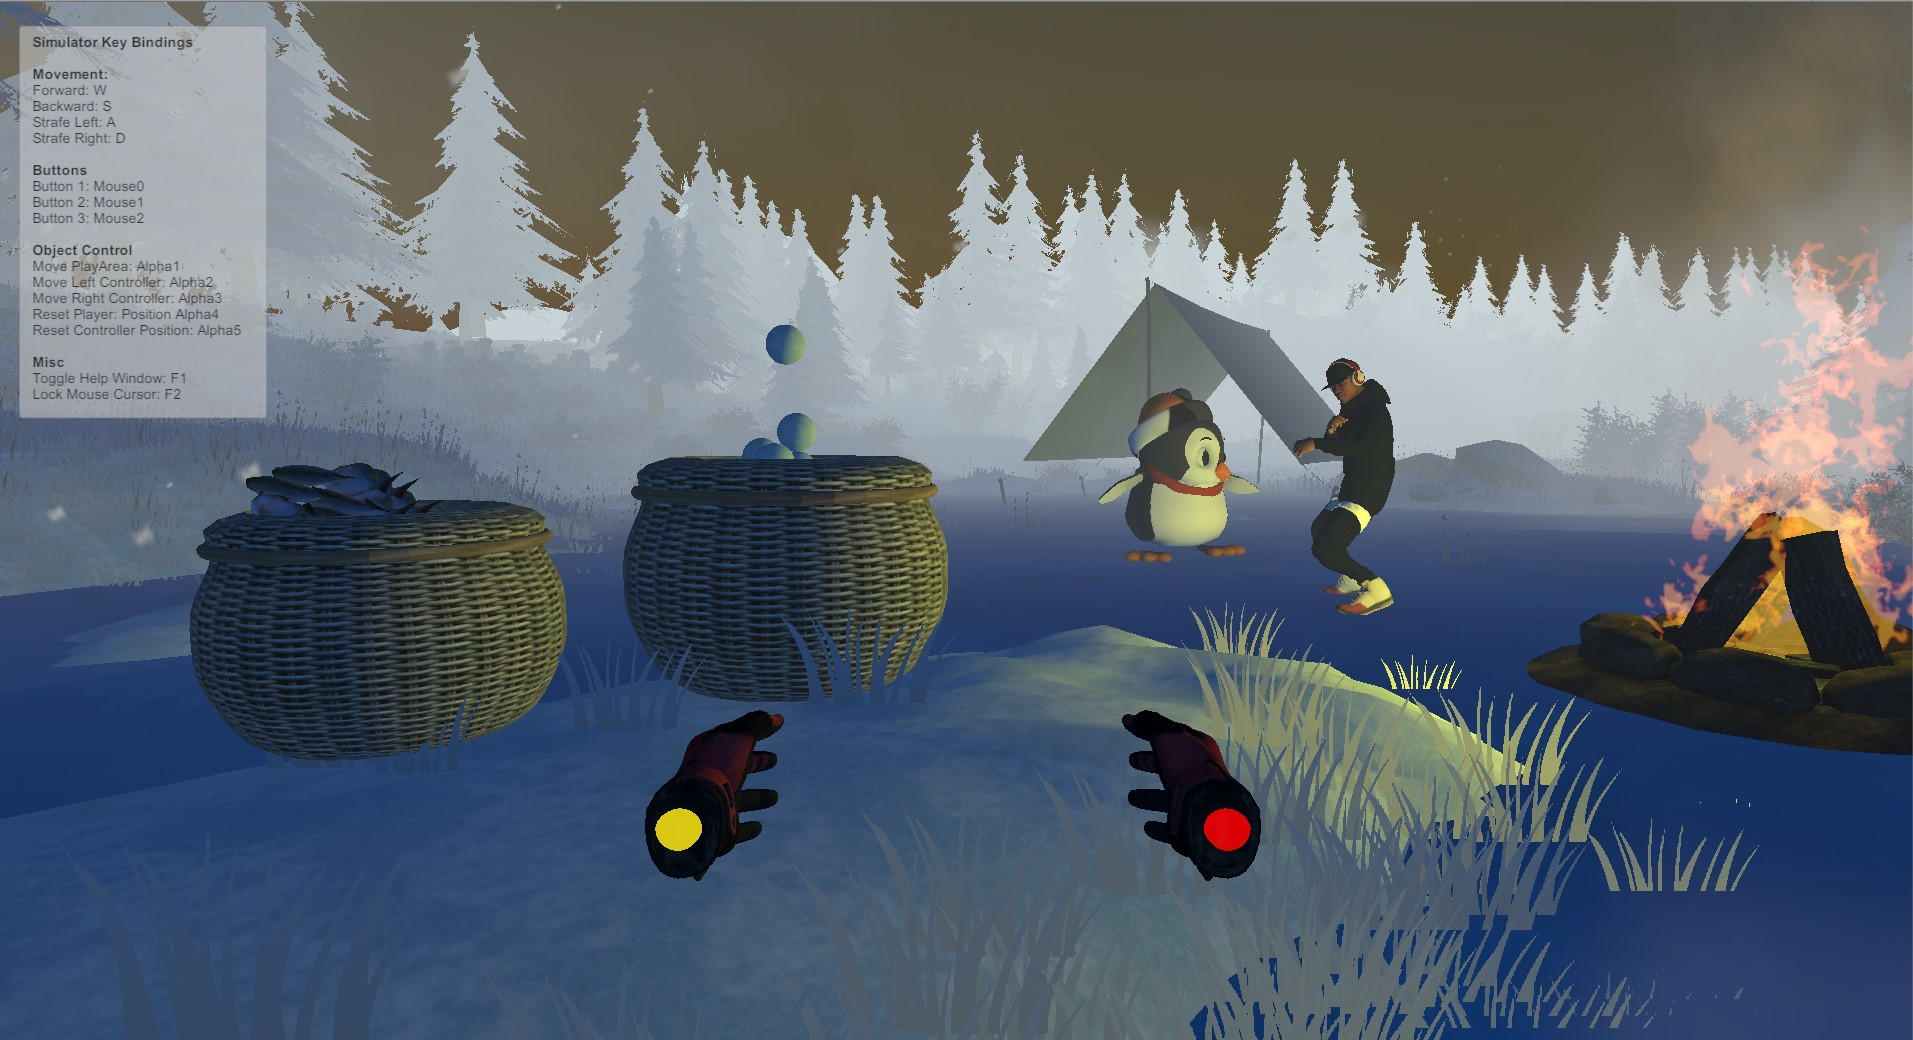
\includegraphics[width=0.75\columnwidth]{./img/peni/draka_obosraka.jpg}
\centering
\caption{Сцена драки, инициированная посредством голосового ввода}
\label{pic:draka}
\end{figure}

\begin{figure}[h]
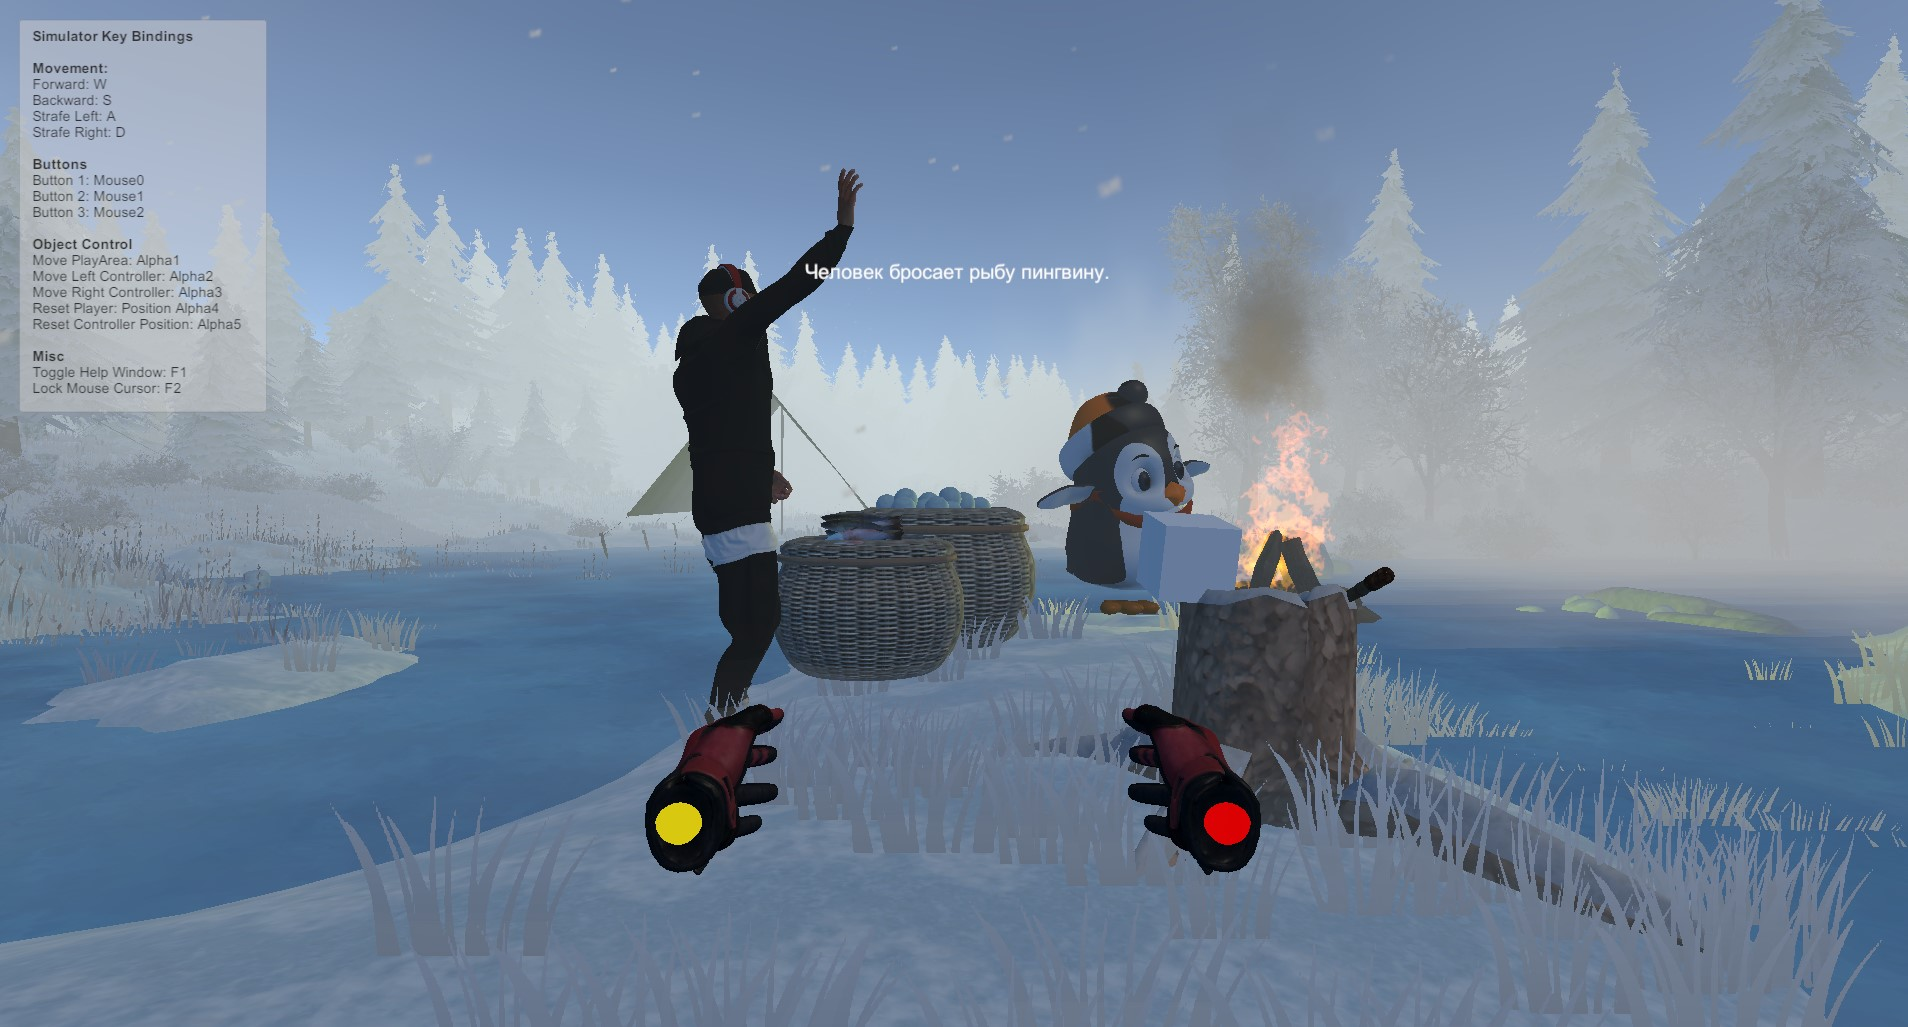
\includegraphics[width=0.75\columnwidth]{./img/peni/kormejka.jpg}
\centering
\caption{Сцена кормежки, инициированная посредством голосового ввода}
\label{pic:kormejka}
\end{figure}

\begin{figure}[h]
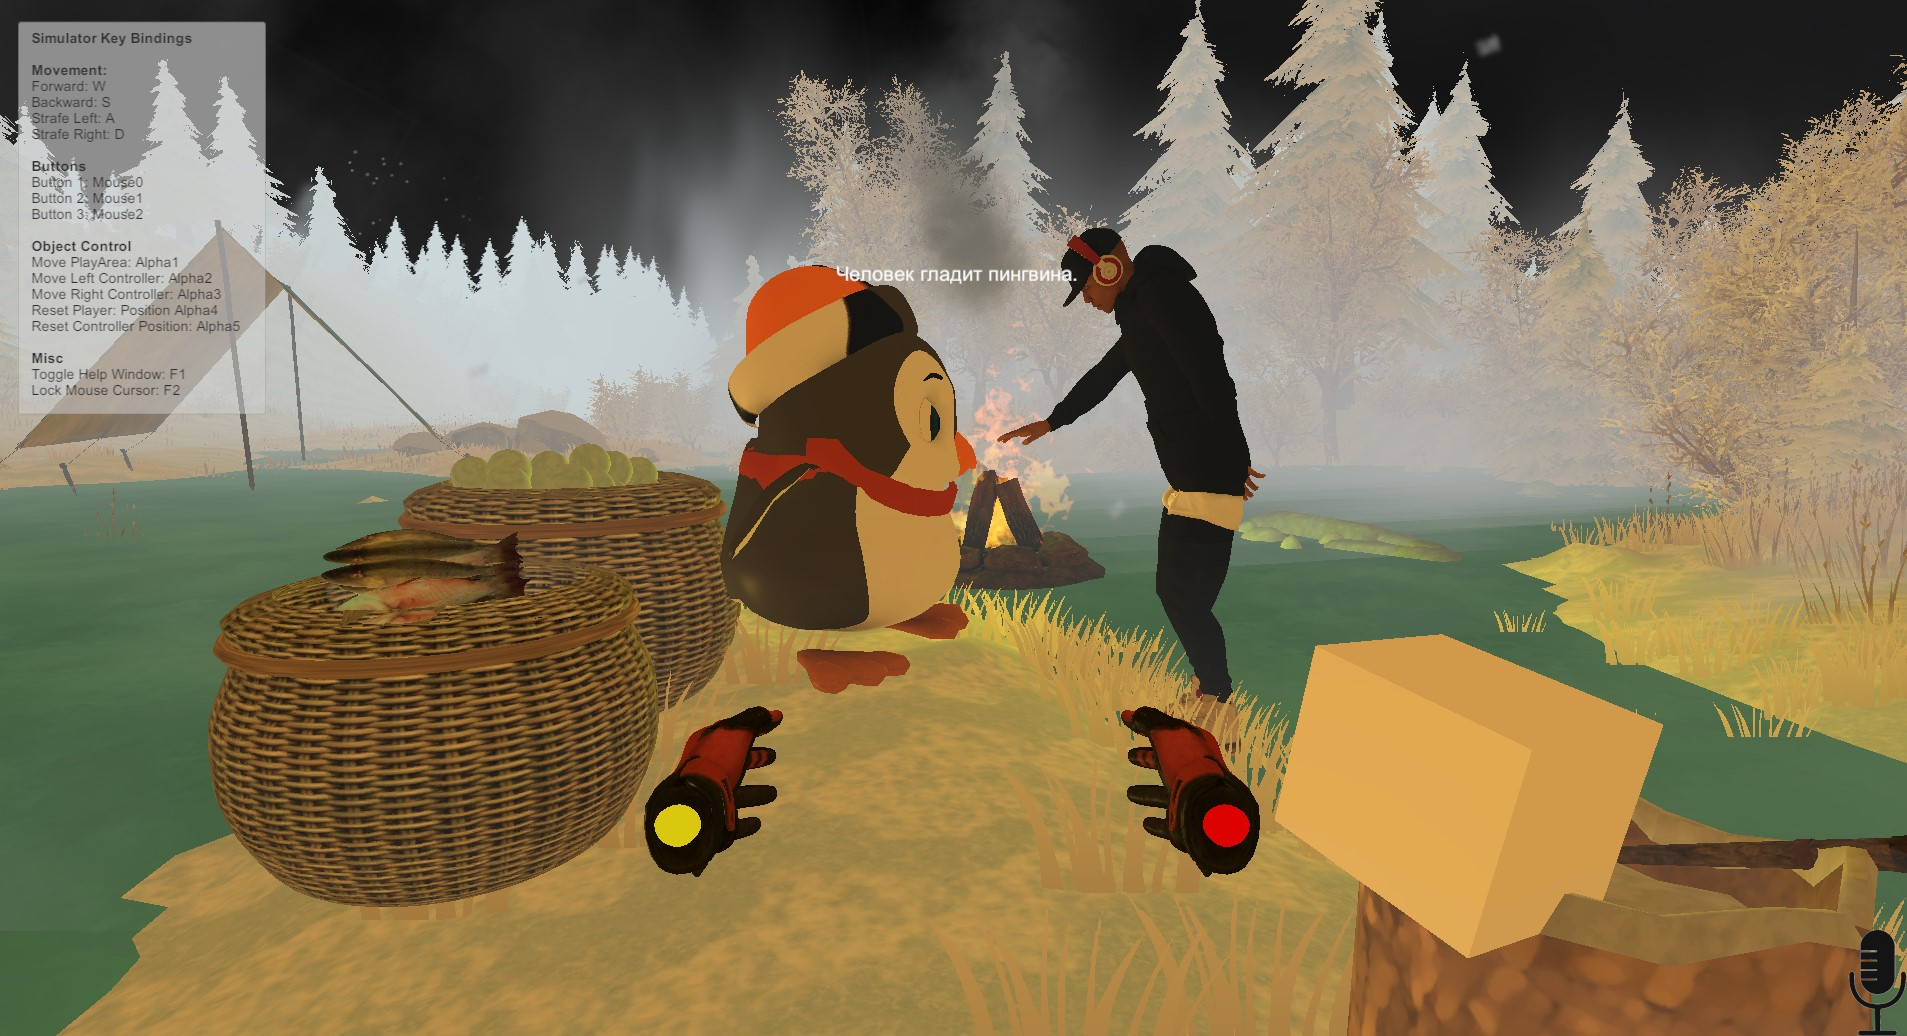
\includegraphics[width=0.75\columnwidth]{./img/peni/nejnost.png}
\centering
\caption{Сцена проявления нежности со стороны человека, инициированная посредством голосового ввода}
\label{pic:nejnost}
\end{figure}

\begin{figure}[h]
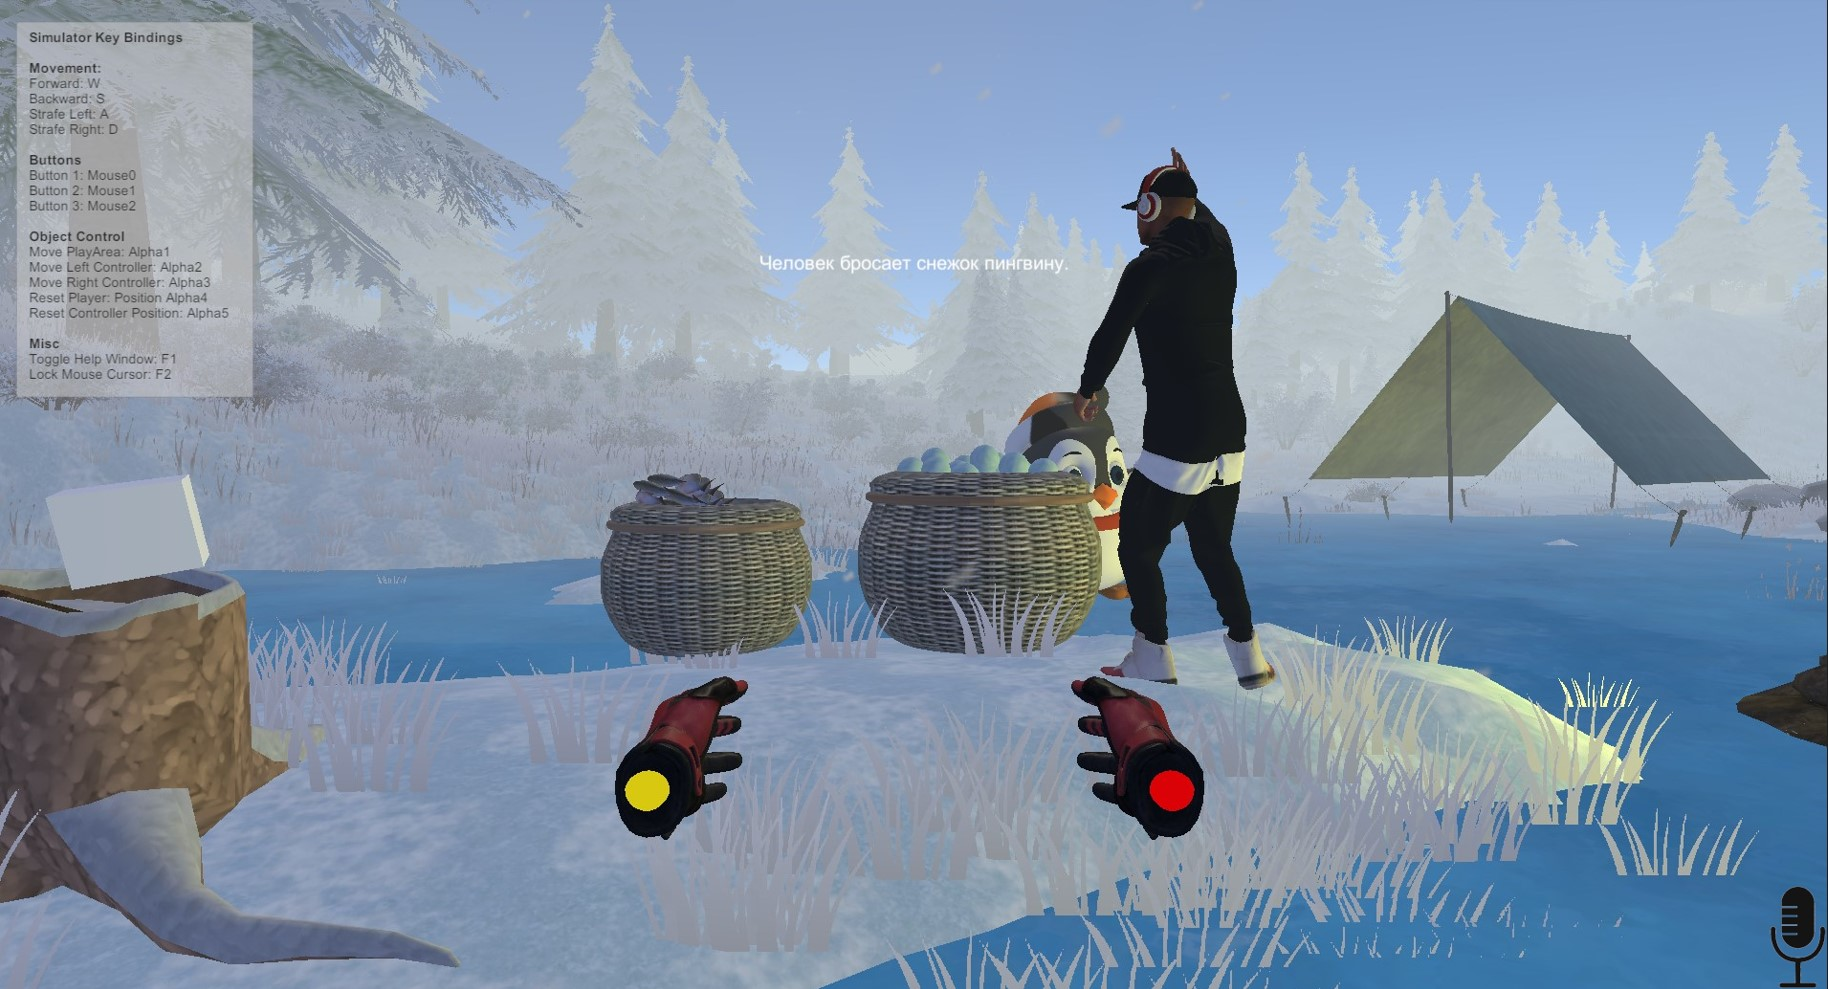
\includegraphics[width=0.75\columnwidth]{./img/peni/snejok.jpg}
\centering
\caption{Сцена игры в снежки, инициированная посредством голосового ввода}
\label{pic:snejok}
\end{figure}

Картинки выше иллюстрируют взаимодействие пингвина с человеком и испытуемым, 
где человек оказывает влияение на акторов посредством ввода голосовых команд.

\section{Выводы}

Было реализовано приложение позволяющее взаимодействовать с виртуальным окружением, в частности с виртуальным актором. 
Были дообучены модели машинного обучения с целью построения эмоционального взаимодействия. 
Для чего в приложение были интегрированы различные технические средства.
